\section{Описание практической части}
\label{sec:Chapter4} \index{Chapter4}

\subsection{Общая схема работы анализатора}

Разработанный инструмент SVAN-FSM реализует сквозной процесс автоматического обнаружения, извлечения и анализа конечных автоматов из описаний на языке SystemVerilog. Общая схема работы инструмента представлена на Рисунке 1. Процесс состоит из следующих этапов:

\begin{enumerate}
\item \textbf{Построение АСД.} Исходный код на SystemVerilog разбирается библиотекой slang [15].
В результате строится абстрактное синтаксическое дерево, содержащее все конструкции исходного кода,
информацию о типах, именах и положениях выражений.

\item \textbf{Трансляция в RTLIL.} АСД транслируется во внутреннее представление Yosys --- RTLIL ---
с помощью yosys-slang [16].

\item \textbf{Обнаружение и извлечение автоматов.} Расширенная реализация проходов fsm\_detect
и fsm\_extract выполняет поиск конечных автоматов в RTLIL-представлении, идентифицирует их входы,
выходы, состояния и переходы, и извлекает каждый автомат в отдельную компактную ячейку \$fsm.

\item \textbf{Графовый анализ.} Каждый извлечённый автомат преобразуется в направленный граф
с использованием библиотеки Boost Graph Library. Полученный граф последовательно проходит
несколько стадий анализа, в ходе которых выявляются мёртвые переходы, недостижимые состояния,
дедлоки и лайвлоки.

\item \textbf{Сопоставление с исходным кодом.} Устанавливается соответствие между элементами АСД
(символами, выражениями) и элементами netlist (проводами, сигналами). Это соответствие позволяет
восстановить имена состояний, условия переходов и ссылки на исходный код в граф-представлении
автомата.
\end{enumerate}

\begin{figure}[h!]
    \centering
    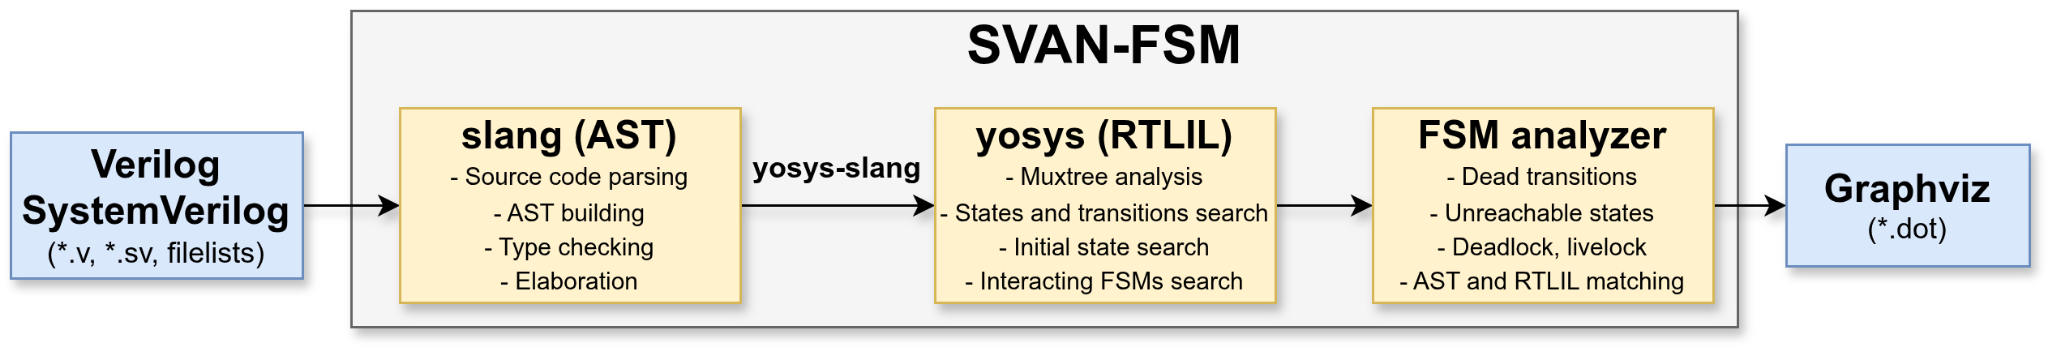
\includegraphics[width=1\linewidth]{images/svan-fsm scheme.png}
    \caption{Общая схема работы разработанного анализатора конечных автоматов}
    \label{fig:placeholder}
\end{figure}

\subsection{Извлечение конечных автоматов из списка логических элементов}

Базовая схема извлечения автоматов, предложенная в Yosys (проходы fsm\_detect и fsm\_extract),
была расширена для устранения ряда практических ограничений, сказывающихся на применимости
инструмента в реальных RTL-проектах. Ниже описаны три ключевых расширения.

\subsubsection{Разбиение проводов на части}

Взаимно-однозначное соответствие между D-триггерами и проводами в netlist соблюдается не всегда.
Рассмотрим типичный случай: в исходном коде объявлен массив состояний

\begin{lstlisting}
state_t state_arr [N-1:0];
\end{lstlisting}

где каждый элемент массива содержит логику отдельного автомата. После преобразования в netlist
для каждого элемента создаётся свой D-триггер, однако все триггеры могут разделять общий провод
(например, если массив объявлен как общий регистр). Это приводит к отображению «многие к одному»:
несколько триггеров отображаются на один и тот же провод. Аналогичная ситуация возникает, когда
регистр состояния встроен в более крупную структуру (например, в packed struct или в более широкий
регистр), и на провод приходится лишь фрагмент, соответствующий конкретному автомату.

Для решения этой задачи реализован механизм, названный разбиением проводов на части (wire blasting).
При обнаружении триггера-кандидата в регистр состояния соответствующий фрагмент общего провода
отделяется и заменяется новым, независимым проводом. Это восстанавливает взаимно-однозначное
соответствие между триггером и проводом, после чего стандартный алгоритм извлечения работает
корректно.

Реализация механизма проверяет, что используется именно фрагмент провода, а не весь провод целиком
(иначе операция не нужна), и что после разделения сохраняются все входящие и исходящие связи.
Операция разбиения выполняется один раз для каждого кандидата и не влияет на общую вычислительную
сложность алгоритма.

\subsubsection{Поддержка автоматов Мили}

Исходная реализация Yosys ограничивается автоматами Мура: функция выходов может зависеть только
от текущего состояния. Эта проверка выполняется в проходе fsm\_detect и отбрасывает автоматы
Мили, встречающиеся во многих реальных проектах.

Расширение анализатора для поддержки Мили основано на следующем наблюдении: для обнаружения
рассматриваемых видов ошибок (мёртвые переходы, недостижимые состояния, дедлоки, лайвлоки)
функция выходов несущественна — анализу подлежит только граф переходов между состояниями.
Поэтому при обработке кандидата в автомат Мили мы отбрасываем зависимые от входов выходы,
сохраняя лишь переходы между состояниями. Это позволяет обрабатывать все автоматы
единообразно --- как Мура --- и одновременно повышает производительность
(меньше данных для обработки).

Модификация реализована на уровне прохода fsm\_detect: условие, требовавшее исключительной
зависимости выходов от состояния, заменено на фильтрацию выходов с последующим их удалением
из \$fsm-ячейки. Функции переходов при этом строятся, как и для автомата Мура, через перебор
состояний и <<вычисление>> комбинационной логики.

\subsubsection{Обработка синхронного сигнала сброса}

В Yosys синхронные и асинхронные регистры обрабатываются по-разному. Для асинхронных регистров
сброс реализуется специальной ячейкой \$adff[TODO],
в которой сигнал сброса передаётся отдельным входом.
Это позволяет алгоритму обнаружения автомата исключить сигнал сброса из рассмотрения и корректно
определить начальное состояние (значение, в которое регистр переходит при активном сбросе).
Для синхронных регистров сброс встроен в мультиплексорное дерево, подаваемое на D-вход обычной
ячейки D-триггера. В этом случае сигнал сброса попадает в число входов автомата, что вызывает
несколько проблем:

\begin{itemize}
\item Появляются дополнительные переходы из каждого состояния в начальное, активируемые
сигналом сброса.

\item Число входов автомата искусственно увеличивается на единицу, что усложняет последующий анализ.

\item Нетривиальным становится определение самого начального состояния, поскольку Yosys в
общем случае не решает эту задачу.
\end{itemize}

Последняя проблема особенно важна, поскольку без знания начального состояния невозможно проверять
достижимость состояний и наличие дедлоков/лайвлоков.

Для корректной обработки синхронного сброса предложен следующий алгоритм. При обходе
мультиплексорного дерева, начиная от корневого мультиплексора, подсчитывается число достижимых
состояний в каждом поддереве. Если ровно одно из поддеревьев корневого мультиплексора содержит
единственное состояние, то это состояние
интерпретируется как начальное, а ветвь управления, активирующая соответствующий вход
мультиплексора, --- как сигнал сброса. Оставшаяся ветвь становится новым корнем мультиплексорного
дерева, и дальнейший анализ уже не зависит от сигнала сброса.

Алгоритм гарантирует корректное восстановление начального состояния в широком классе реальных
RTL-описаний и приводит обработку синхронно сбрасываемых регистров к тому же виду,
что и асинхронных.

Сложность процедуры извлечения автомата определяется в первую очередь построением таблицы переходов
в проходе fsm\_extract. Для каждого из $|S|$ возможных состояний схема вычисляется путём перебора
комбинаций входов до тех пор, пока все переходы не будут определены. В худшем случае это даёт
сложность $O(|S|\cdot 2^{|I|}\cdot|M|)$, где $|I|$ — число входов автомата, $|M|$ — размер
мультиплексорного дерева. На практике, однако, $|I|$ обычно невелико (порядка десятков), а ранние
завершения при определении переходов существенно сокращают число требуемых итераций.

\subsection{Графовый анализ конечного автомата}

После извлечения каждый конечный автомат преобразуется в графовое представление и
последовательно подвергается трём стадиям анализа. Каждая стадия уточняет граф, удаляя
из него заведомо некорректные элементы, что повышает точность последующего анализа.
На Рисунке 2 показан модельный пример графа автомата с размеченными ошибками и
соответствующий ему исходный код на Verilog.

\begin{table}[h!]
    \centering
    \begin{tabular}{|c|l|}
    \hline
\begin{lstlisting}
`define INIT 0
`define S1 1
`define S2 2
`define S3 3
`define S4 4
 
module top (input clk, ctl, rst,
            output reg outp);
  reg [2:0] state;
  always @(posedge clk) begin
    if (rst) begin
      state <= `INIT;
      outp  <= 1'b0;
    end else case (state)
      `INIT: state <= `S1;
      `S1: begin
        state <= `S2;
        outp  <= 1'b1;
      end
      `S2: if (ctl)
           state <= `S3;
      `S3: if (ctl & !ctl)
             state <= `S4;
           else state <= `S3;
      `S4: state <= `INIT;
    endcase
  end
endmodule
\end{lstlisting}
         &
\makecell[lt]{
    
\includegraphics[width=0.35\linewidth]{example.png} \\ ~ \\
    Состояния: \\
    \textcolor{green}{$\blacksquare$} начальное состояние \\
    \textcolor{red}{$\blacksquare$} недостижимое состояние \\
    \textcolor{blue}{$\blacksquare$} дедлок \\
    \textcolor{violet}{$\blacksquare$} лайвлок \\ ~ \\
    Переходы: \\
    \textcolor{orange}{$\blacksquare$} \textcolor{red}{$\blacksquare$} мёртвый переход \\
}
         \\ \hline
    \end{tabular}
    \caption{Граф конечного автомата с размеченными ошибками (справа) и соответствующий ему
    Verilog-код (слева)}
    \label{tab:placeholder}
\end{table}

\subsubsection{Обнаружение мёртвых переходов}

На первой стадии анализа выполняется поиск мёртвых переходов. В текущей реализации обнаружение
основано на выявлении противоречий, связанных с входами автомата, имеющими константные значения.
Константные значения входов могут возникать по нескольким причинам: явное присваивание константы
в исходном коде, значения параметров, подставленные при элаборации модуля, или результат
оптимизаций синтеза (например, распространение констант, удаление недостижимых ветвей).

Алгоритм работает следующим образом. Сначала при обходе netlist определяются все входы автомата,
жёстко привязанные к логическим 0 или 1. Затем для каждого перехода его условие реконструируется
как конъюнкция атомарных предикатов над входами. Если хотя бы один из предикатов противоречит
известному константному значению входа (например, условие требует значения '1', тогда как вход
постоянно равен '0'), переход классифицируется как мёртвый и удаляется из графа.

Несмотря на простоту, метод эффективен на практике: в реальных проектах константные входы возникают
повсеместно, особенно в параметризованных модулях и после распространения констант при оптимизации.
Удаление мёртвых переходов существенно повышает точность последующего анализа достижимости и сильно
связных компонент.

Более точное определение недостижимости переходов требует рассуждений над отношениями между
непостоянными входами, что в общем случае эквивалентно задаче удаления мёртвого кода и является
вычислительно дорогостоящим. Интеграция методов SAT-решения или символьного исполнения оставлена для
будущих работ.

\subsubsection{Анализ недостижимых состояний}

На второй стадии выявляются недостижимые состояния. Недостижимые состояния определяются поиском
в ширину (англ. breadth-first search, BFS) по графу, стартующим из начального состояния.
Состояние классифицируется как недостижимое, если в него невозможно попасть ни по какому
пути из начального состояния.

Существенно, что анализ работает на графе, из которого уже удалены мёртвые переходы. Это
повышает число обнаруживаемых проблем и общую точность анализа: состояние, достижимое лишь
через мёртвый переход, после удаления этого перехода окажется полностью изолированным и будет
корректно классифицировано как недостижимое. В противном случае такое состояние ошибочно
считалось бы достижимым.

\subsubsection{Обнаружение дедлоков и лайвлоков}

На третьей стадии обнаруживаются дедлоки и лайвлоки. Анализ основан на нахождении сильно
связных компонент (ССК) с помощью алгоритма Тарьяна, имеющего временную сложность
$O(|V| + |E|)$, где $|V|$ и $|E|$ --- число вершин и рёбер графа соответственно. Следуя
определениям, данным в разделе 4.1.4, каждая найденная ССК проверяется на наличие исходящих
рёбер, ведущих в вершины вне компоненты. Если таких рёбер нет и компонента не является
главной группой (содержащей начальное состояние), она классифицируется как ТССК.

Анализ выполняется на графе, из которого уже удалены мёртвые переходы и недостижимые состояния,
что обеспечивает корректность результатов: все оставшиеся компоненты заведомо достижимы из
начального состояния. ТССК, содержащая единственную вершину, классифицируется как дедлок;
ТССК, содержащая несколько вершин, --- как лайвлок.

Результаты анализа экспортируются в файл формата DOT (Graphviz) с разметкой: начальное состояние выделяется зелёным контуром, недостижимые — фиолетовым, дедлок — красным, лайвлок — оранжевым (см. Рисунок 2). Условия переходов выводятся в виде формулы в дизъюнктивной нормальной форме, реконструированной из атомарных входов автомата.

\subsection{Сопоставление результатов анализа с исходным кодом}

Для повышения удобства использования инструмента каждый конечный автомат представляется в виде
направленного графа, в котором вершины — это состояния, а рёбра — переходы. Вершины помечаются
именами состояний, заданными в исходном коде (как правило, через enum или parameter), а рёбра ---
условиями переходов, выраженными через оригинальные имена сигналов и констант. Поскольку на уровне
netlist информация об исходном коде частично теряется, требуется специальная процедура сопоставления
элементов АСД и netlist. Эта процедура реализована в виде двух последовательных проходов.

\subsubsection{Отображение входов конечного автомата на выражения АСД}

Первый проход, fsm\_match\_conditions, устанавливает соответствие между входами извлечённого
конечного автомата и выражениями из АСД. Для обеспечения такого соответствия был существенно
изменён формат атрибута src в RTLIL, в котором хранится информация о местоположении элементов
в исходном коде.

Первое изменение касается способа хранения позиции. Поскольку библиотека slang не позволяет
восстановить объект SourceLocation по имени файла и текстовой позиции, в новом формате src
хранится пара: BufferId (идентификатор буфера, в котором хранится файл) и Offset (смещение
в байтах относительно начала буфера) --- с помощью которой однозначно восстанавливается AST-символ,
соответствующий данному проводу.

Второе изменение — поддержка посимвольной разметки. Один и тот же провод может соответствовать
нескольким АСД-символам (например, если он образован из полей упакованной структуры).
Поэтому новый формат src хранит информацию о местоположении не только для всего провода
целиком, но и для отдельных его битовых срезов. Это позволяет корректно сопоставлять вход
автомата с конкретным полем структуры в исходном коде.

Третье изменение — распространение src при соединениях. Когда в netlist соединяются два провода
(например, при инстанцировании модуля), их атрибуты src наследуются друг от друга. Это
обеспечивает непрерывность связи с исходным кодом даже сквозь границы модулей и
промежуточные сигналы.

В совокупности эти изменения позволяют реализовать обход АСД, который собирает все условные
конструкции (if, тернарные операторы, блоки case) и сопоставляет их местоположения с
местоположениями входов автомата. В результате каждому входу автомата ставится в соответствие
исходное выражение, что позволяет в дальнейшем выводить условия переходов в осмысленном виде.

\subsubsection{Восстановление имён состояний}

Второй проход, fsm\_analyze, восстанавливает имена состояний. Задача эта нетривиальна, поскольку
в реальных автоматах логика часто распределена по нескольким переменным: например, отдельно
объявляется регистр состояния (state) и переменная следующего состояния (next\_state), причём
присваивание из next в current происходит в отдельном always\_ff блоке или через порт
инстанцируемого модуля триггера.

Алгоритм восстановления имён состоит из трёх шагов:

\begin{enumerate}
\item Для каждого АСД-символа собираются именованные константы, которые ему присваиваются или
с которыми он сравнивается, а также другие символы, присваиваемые ему (в том числе через порты
модулей).

\item Итеративно выполняется распространение присваиваний: каждый символ расширяет своё множество
ассоциированных констант и символов, добавляя множества от всех символов, на которые он ссылается.
Алгоритм конечен и сходится за число шагов, не превышающее размера графа ссылок.

\item Для каждого извлечённого конечного автомата соответствующий ему АСД-символ восстанавливается
по иерархическому имени, и имена состояний берутся из полученного множества констант.
\end{enumerate}

Между fsm\_match\_conditions и fsm\_analyze запускаются оптимизационные проходы Yosys (opt).
Эти оптимизации могут увеличить число константно-значных входов автомата и тем самым раскрыть
дополнительные мёртвые переходы. Однако оптимизации могут также отбрасывать метаданные о
местоположении в исходном коде. Двухпроходная архитектура решает эту проблему:
fsm\_match\_conditions фиксирует все необходимые сопоставления до оптимизаций, после чего
потеря части src-информации уже не влияет на качество анализа.

\subsection{Обнаружение взаимодействующих автоматов}

В реальных RTL-проектах управляющая логика редко реализуется в виде одного изолированного
конечного автомата. Чаще встречается сценарий, при котором несколько автоматов взаимодействуют
для реализации протоколов, конвейеров или цепочек управления. При этом ошибки в таких системах
часто возникают не в отдельных автоматах, а именно во взаимодействии между ними. Это мотивирует
разработку автоматического обнаружения зависимостей между конечными автоматами.

Формально мы определяем два автомата как взаимодействующие, если сигнал, генерируемый одним
автоматом, достигает логики переходов другого автомата через путь, содержащий произвольную
комбинационную логику и не более одного регистра.

Для обнаружения таких взаимодействий анализатор выполняет обход вперёд, начиная от каждого
выхода конечного автомата. В процессе обхода допускается прохождение через любое число
комбинационных элементов, тогда как через триггеры разрешается проходить не более одного раза.
Всякий раз, когда достигается вход другого автомата, между соответствующими экземплярами
автоматов фиксируется направленная зависимость. Обход имеет линейную по размеру netlist сложность
и вносит пренебрежимо малые накладные расходы по сравнению с извлечением автомата.

Обнаружение взаимодействующих автоматов даёт несколько важных преимуществ. Во-первых, оно помогает
разработчику понять архитектурные управляющие зависимости, что особенно ценно в больших проектах,
содержащих десятки автоматов. Во-вторых, информация о взаимодействиях может комбинироваться с
диагностикой на уровне отдельных состояний: например, условие дедлока или лайвлока в одном
автомате может распространяться на зависимые автоматы, что позволяет локализовать первопричину
ошибки в одном блоке управления и её проявления в других. В-третьих, циклические зависимости
в графе взаимодействий могут указывать на архитектурные проблемы, такие как
непреднамеренная обратная связь между контроллерами.
